% 2.	Objectifs / Objectives: ½ page

\hspace*{0.3cm}

\noindent We now discuss the current state of the art of the research at hand. There are two main points to address in this respect; the first one relates to the current state of seismic source inversion, and the second one addresses the state of  multi-level and multi-index Markov chain Monte Carlo methods. The former has been traditionally dominated by deterministic inversion, with the use of the more robust, MCMC based probabilistic inversion having been recently introduced. The latter tries to extend the ideas of multi-level and multi-index Monte Carlo to an MCMC setting. This in turn is still at a very early stage, with only a handful of papers discussing this ideas.  

 \subsection{Seismic  Inversion}
\color{blue} Some things in this section borrow form the CRG4 grant proposal...How can I cite that? \color{black}
In earthquake  inversion, we try to estimate the material properties (such as velocity, density and Lam\'e parameters) or the kinematic parameters of the earthquake rupture process that occurs on a geological fault plane of finite spatial extent (finite-fault) within the earth. These parameters can be the point-source location, the  spatially variable displacement across the fault surface (slip), the slip direction, the slip duration (which is tied to a poorly known slip-rate function), and the rupture time (time at which each point on the fault starts to slip; this is tied to a rupture velocity). To this end, seismologists have developed numerous techniques over the past decades.  Traditionally, a deterministic approach has been employed, on which a misfit  functional $J(\te)$ (where $\te$ represents the vector of parameters of interest) measuring the difference between some recorded data $y$ and some generated data $\mathcal{F}(\te)$ is defined and minimized. Thus the deterministic inversion reads as a constrained optimization problem $$\min_{\te \in \bm{\Omega}} \Phi(\te)$$ with $$\Phi(\te)=J(\te)-\frac{\alpha}{2}R,\quad \text{such that (\ref{strongform}) holds}, $$  where $R$ is a regularizing term (such as Tykhonov or total variation) and $\alpha$ is  some regularization parameter. This approach has been studied extensively \cite{hormander1985analysis,komatitsch1999introduction} and it is still a fairly active area of research in the geophysics community, however, these methods are prone to discrepancies \cite{beresnev2003uncertainties}. An example can be seen for the 2011 Tohoku earthquake (Japan), where a survey over more than 20 different inversion methods described in various papers  yields widely different results for the source location (see, for example, \cite{hayes2011rapid,shao2011focal,SRCMOD}). This calls for models that can  accurately quantify  uncertainty.\begin{figure}[H]
	\centering
	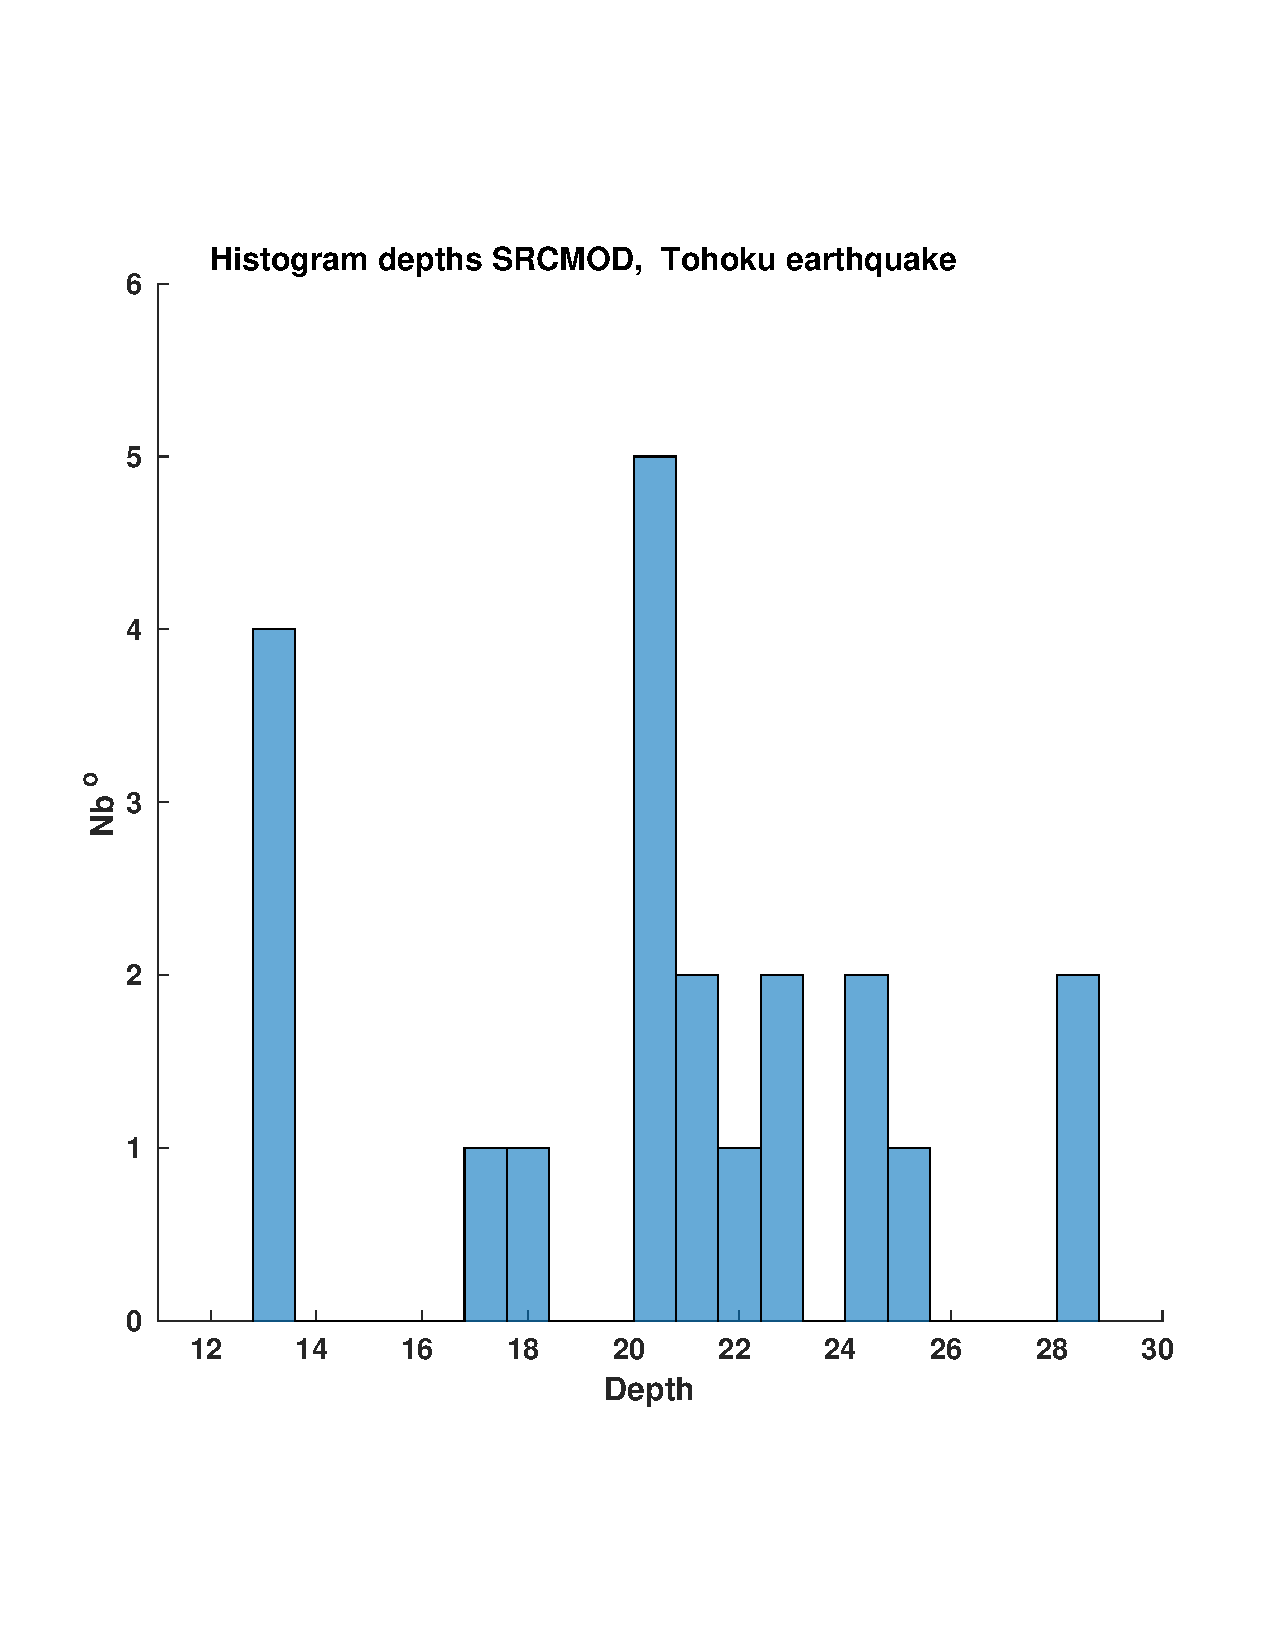
\includegraphics[width=0.5\linewidth]{figures/HistogramTohoku}
	\caption{Histogram of different source locations obtained for the 2011 Mw 9.0 Tohoku earthquake.}
	\label{fig:histogramtohoku}
\end{figure}



 \noindent More recently,  full Bayesian estimation of earthquake  properties has been attempted (see, for example \cite{minson2013bayesian,bui2013computational}) although it is still in its early stages and geared mostly towards inversion on the material properties of the medium, rather than on the physical properties of the earthquake.  This lack of development of this type of methods is mostly linked to the large cost associated to obtaining numerical simulations of the  forward problem of local, regional, or global seismic wave propagation. To mitigate this computational burden, various simplifying assumptions are typically made. Thus, a complete or comprehensive quantification of the uncertainties in the resulting finite-fault rupture models, owing to (a) data errors; (b) unknown earth structure; (c) unknown rupture physics (e.g. detailed fault geometry; poorly known slip-rate function); (d) simplification in computing the response functions is still missing in the literature. 
 
 \subsection{Markov Chain Monte Carlo}

\subsection{Muti-level and Multi-index Markov Chain Monte Carlo}
The work done on ML/MI-MCMC is still on its very early stages, with only a handful of papers on the topic \cite{dodwell2015hierarchical,hoang2013complexity,jasra2018multi} , focusing mostly on inverse problems involving elliptic PDEs. To the best of our knowledge, there has not been a rigorous attempt to extend these methods to inverse problems involving hyperbolic PDEs. Moreover, the algorithms discussed therein are open to improvements. To better understand the theory behind these methods, we first discuss briefly the ideas underlying  MLMC and MIMC, as ML/MI-MCMC are an extension of these to MCMC.  MLMC are algorithms for computing expectations that arise in stochastic simulations in cases in which the stochastic model can not be simulated exactly, rather approximated at different levels of accuracy and as such, at different computational costs. Just as Monte Carlo methods, they rely on repeated random sampling, but these samples are taken on different levels $\ell$ of accuracy (cheap simulations), in such a way that the majority of the samples $M_\ell$ are obtained with low accuracy. In the case of PDE driven inverse problems, this can be understood as introducing a hierarchy of discretizations $\{h_\ell\}_{\ell=0}^L$ such that the cost of solving the PDE and the accuracy of the numerical solution increase as $\ell$ increases. %By following an idea similar to that of multi-grid algorithms, where the majority of the samples are obtained  at  coarser discretizations, 
 MLMC methods can greatly reduce the computational cost of standard Monte Carlo methods by taking most of the samples at a low accuracy and corresponding low cost, and only very few samples  at high accuracy and corresponding high cost.   In the standard MLMC approach we denote the resulting approximation of a quantity of interest using mesh size $h_\ell$ in the simulation of a forward observation  operator event by $\QoI_\ell(\te)$ . Then, the expected value of the finest approximation, $\QoI_L$, can be expressed as
\begin{align*}
%\label{eq:telescoping}
\E[{\QoI_L}] & =
\E[\QoI_0] + \sum_{\ell=1}^L \E[\QoI_{\ell}-\QoI_{\ell-1}],
\end{align*}
and the MLMC estimator is obtained by approximating the expected values
in the telescoping sum by sample averages as
\begin{align}
\label{eq:MLMC_estimator}
\mathcal{A} & = \frac{1}{M_0}\sum_{m=1}^{M_0}\QoI_0(\te_{0,m}) +
\sum_{\ell=1}^L\frac{1}{M_\ell}\sum_{m=1}^{M_\ell}
\left(\QoI_{\ell}(\te_{\ell,m})-\QoI_{\ell-1}(\te_{\ell,m})\right),
\end{align}
where, for every $\ell$,  $\{\te_{\ell,m}\}_{m=1}^{M_\ell}$
denotes independent identically distributed (i.i.d.) realizations of the mesh-independent random variables $\te$. If $W_\ell$ is the average cost associated with generating one sample of the difference, $\QoI_{\ell}-\QoI_{\ell-1}$, or simply $\QoI_0$ if $\ell=0$, then the cost of the
estimator~\eqref{eq:MLMC_estimator} is
\begin{align}
\label{eq:work_sum}
\work & = \sum_{\ell=0}^{L} M_\ell W_\ell.
\end{align}
%
We assume that the work required to generate one sample of mesh size
$h$ is proportional to $h^{-\gamma}d$, where $d$ is the dimension of the
computational domain and $\gamma > 0$ represents the complexity of
generating one sample with respect to the number of degrees of freedom.
Thus, we model the average cost on level $\ell$ as
\begin{align}
\label{eq:wl_model}
W_\ell \leq h_\ell^{-\gamma}d,
\end{align}
and consequently use the representation
\begin{align}
\label{eq:model_work}
\work & \leq \sum_{\ell=0}^{L} \frac{M_\ell}{h_\ell^{\gamma}}
\end{align}
for the total work to evaluate the MLMC estimator~\eqref{eq:MLMC_estimator}.
It can be shown that under certain conditions on the ccuracy of the PDE solver and on the variance of the increments, for a given tolerance $\epsilon$, there exist a constant $c_\text{mlmc}$ \begin{align}\label{mlmc_cost}
\E[\work]\leq\begin{cases}
c_\text{mlmc}\epsilon ^{-2}& \beta>\gamma \\
c_\text{mlmc}\epsilon ^{-2}\log(\epsilon)^2& \beta=\gamma \\
c_\text{mlmc}\epsilon ^{-2-(\gamma-\beta)/\alpha}& \beta<\gamma, \\
\end{cases}
\end{align}
where $\alpha$ is related to the numerical accuracy of the PDE solver and $\beta$ is related to the decay rate of the variance of the increments \cite{giles2008multilevel}. A further improvement over the non-optimal regime ($\beta>\gamma$) can be obtained using  multi-index Monte Carlo (MIMC), for which different discretization directions are used \cite{haji2016multi}. These methods have successfully been implemented for a wide variety of problems, including simulation of random paths, option pricing etc. Extending these methods to a MCMC setting is not a trivial task since (i) the MLMCMC algorithm must be constructed in such a way that  samples in two continuous chains are correlated (so that the variance of the increment in $\QoI_\ell$ decays as $\ell$ increases) and the algorithm should, ideally generate samples with a small autocorrelation time within chains, since, as opposed to pure Monte Carlo, MCMC generates samples that are correlated, which will generate a bias on the estimator.  As mentioned before,  only a few works so far have dealt with the ML-MI extension of MCMC methods for posterior exploration in Bayesian inversion. Of theoretical importance is the work of \cite{hoang2013complexity}, as it provides a very thorough analysis to a particular version of these methods applied to inverse problems involving elliptic PDEs. However, the method described in that paper generates proposals based on independent samplers (see \cite{asmussen2007stochastic}), and this in turn can become widely inefficient if the proposal generating function is not constructed carefully. The work of \cite{dodwell2015hierarchical} proposes a more efficient algorithm and provides an estimate for the total work necessary to obtain a tolerance of $\epsilon$, given by a form similar to (\ref{mlmc_cost}). \begin{definition}
	We define the mean squared error (MSE) associated to a MCMC algorithm by $$e^2_{MSE}(\QoI_{\ell})=\E_\vartheta\left[ \left(\frac{1}{M_\ell}\sum_i^{M_\ell}\QoI^i-\E_\mu(\QoI)\right)^2	\right], $$
	where $\QoI$ is some quantity we wish to estimate, following some (unachievable) distribution $\mu$ and where $\vartheta$ is the distribution from which we are actually able to sample.  \end{definition} 

\begin{definition}
	Suppose each sample at level $\ell$ has an associated cost $\mathcal{W}_\ell$. We denote the $\varepsilon$-cost, i.e, the cost associated to obtaining a mean squared error of $\varepsilon$ when estimating $\QoI$ by $\mathcal{W}_\ell^\epsilon(\QoI).$ 
\end{definition}
\begin{theorem}
Denote by $Y_\ell=$	Suppose that all chain have been sufficiently burned-in and that there exist $\alpha,\beta,\gamma>0$, and $\varepsilon<e^{-1}$, such that $\alpha\geq\min(\beta,\gamma)$. Suppose the following assumptions hold for all $\ell\geq 0 $: \begin{enumerate}
		\item[i)] $\lv \E_{\pi_{\ell,h}}[Q]-\E_{\pi_\ell[Q]}\rv \leq C_1 h_\ell^{\alpha  }$
		\item[ii)] $\V_{\pi_{\ell,h}}[Y_\ell]\leq C_2 h_\ell^{\beta}$
		\item[iii)] $e_\text{MSE}(Y_\ell)\leq C_3 \sup|\V_{\ell}[Y_\ell]|M_\ell^{-1/2}$
		\item[iv)] $W_\ell^\epsilon(\QoI)\leq C_4h_\ell^{-\gamma},$
	\end{enumerate}
	then, there exist a number of levels $L$ and a sequence of $\{N_\ell\}_{\ell=0}^L$ such that $$e(\QoI_{L})\leq\varepsilon,$$ and \begin{align}
	\mathcal{W}_L^\epsilon(\QoI)\leq C_5\begin{cases}
	\varepsilon^{-2}|\log\varepsilon|, & if \ \beta>\gamma,\\
	\varepsilon^{-2}|\log\varepsilon|^3, & if \ \beta=\gamma,\\
	\varepsilon^{-2+(\gamma-\beta)/\alpha}|\log\varepsilon|, & if \ \beta<\gamma.\\
	\end{cases}
	\end{align}
\end{theorem}  



